\chapter{Schlussbetrachtung}

\section{Kritische Reflektion}

Neben den vielen Potenzialen eines dynamischen Learning-NFT und der darunter liegenden Blockchain Technologie gibt es jedoch auch Schattenseiten.

Der Energiekonsum der Blockchain Technologie ist seit seiner Entstehung ein heiß diskutiertes Thema.
Denn für die Transaktionsprüfung sind spezifische kryptografische Probleme zu lösen.
Diese Hashes werden von \dq Minern\dq{} mit speziell designten Computern rund um die Uhr berechnet, was jedoch viele reale Ressourcen wie Rechenleistung und Energie benötigt \parencite[vgl.][]{Cvj.ch.01.04.2022}.
So hat zum Beispiel die Bitcoin Blockchain mit über 5 Millionen Hardwaregeräten einen jährlichen Stromverbrauch von 89 \ac{TWh}.
Klingt erstmal viel, im Vergleich zum weltweiten Energiebedarf von 162.194 \ac{TWh} ist es aber ein lediglich geringer Anteil von 0,05\% \parencite[vgl.][11]{CoinShares.2022}.

Trotz dessen ist es immer noch ein hoher Verbrauch und verursacht jährlich 36 \ac{Mt} CO\textsubscript{2}.
Immer effizienter werdende Computersysteme können den Stromverbrauch und damit auch die CO\textsubscript{2} Emissionen verringern
(siehe Abbildung \ref*{fig:btceff}) haben aber leider nur einen geringen Einfluss.

    \begin{figure}
        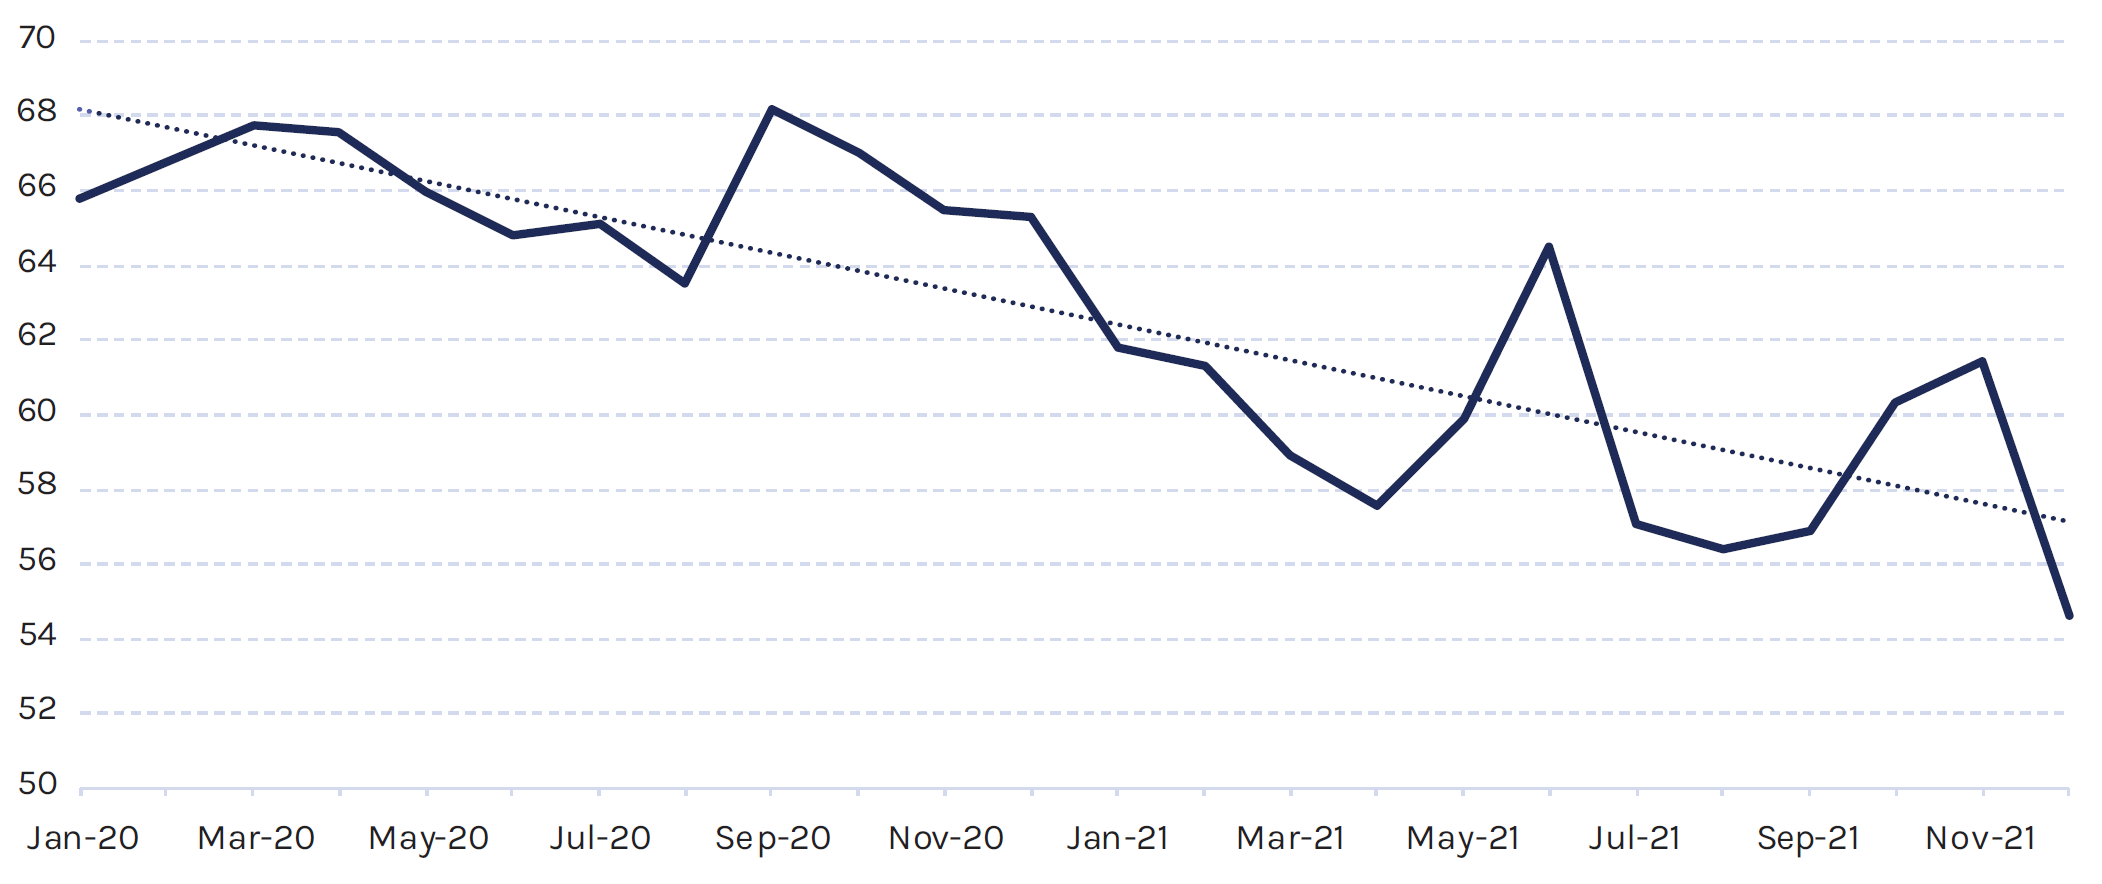
\includegraphics[width=15.8cm]{Bilder/BitcoinEffizienz.PNG}
        \centering
        \captionabove[Effizienz des Bitcoinnetzwerk]{Zeitlicher Verlauf der Effizienz des Bitcoinnetzwerk in Joule pro Tera-Hash \parencite[vgl.][]{CoinShares.2022}}
        \label{fig:btceff}
    \end{figure}

Der hohe Verbrauch der Bitcoin Blockchain ist dabei vor allem auf die Art des Einigungsverfahrens zurückzuführen.
Denn Blockchain arbeitet, wie schon im Grundlagenkapitel erwähnt, mit dem \acf{PoW}, also \dq Beweis durch Arbeit\dq{}.
Eben jene Arbeit ist für den größten Teil des Energiebedarfs zuständig.
Die Blockchain Ether möchte deshalb mit Ethereum 2.0 sein Konsensverfahren von \ac{PoW} auf \acf{PoS} umstellen.
Dieser Prozess ist nicht auf viel Rechenleistung und Energie angewiesen und könnte damit eine grünere Blockchain ermöglichen.
Leider ist bei \ac{PoS} gegenüber \acf{PoW} durch dieses verfahren auch die Manipulation etwas weniger aufwändig und damit ein wenig unsicherer \parencite[vgl.][]{Ginsburg.10.11.2021}.

\section{Fazit}

Abschließend lässt sich sagen, ein Learning-NFT ist ein vielversprechendes Konzept und bietet neue Möglichkeiten nachhaltiges Lernen in verschiedensten Formen zu verbessern, erweitern und steuern zu können.
Für die SAP Experience Garage Technology Plattform ist das Konzept auch sehr interessant, den dynamischen Learning-NFT aber komplett mit allen Bestandteilen umzusetzen ist jedoch nicht sinnvoll.
Wie in Kapitel \ref{testref} beschrieben würde die Implementierung der Methodik und Funktionsweise zum Lernen durch wiederholte Lerneinheiten, in Verknüpfung mit einem Score,
einen großen Wert für Plattform und Nutzer bei geringem Implementierungsaufwand bieten.
Diesen Score in einem NFT abzulegen würde jedoch kaum Nutzen bringen und hohen Zeitaufwand als auch hohe monetäre Kosten für Transaktionen verursachen. 

\section{Ausblick}

Das Konzept von dynamischen Learning-NFTs ist noch in seiner Anfangsphase.
Für die Zukunft lässt sich aber nach Betrachtung dieser Arbeit sagen, dass die Potenziale des Learning-NFTs sehr groß sind und Abseits von der SAP Experience Garage Technology Plattform noch einen deutlich größeren Mehrwert liefern können.
Eine Anwendung wie beispielsweise SAP SuccessFactors \parencite[]{SAP.28.08.2022} oder LinkedIn.